\documentclass[hyperref={colorlinks=false, breaklinks=true},11pt]{beamer}
%\usepackage[utf-8]{inputenc}
%\usepackage[english,russian]{babel}
\usepackage{graphicx}
\usepackage{longtable}
\usepackage{listings}
\usepackage{latexsym}
\usepackage{psfrag}
\usepackage{helvet}
\usepackage{url}
\usepackage{romannum}

%\usetheme{default}
%\usefonttheme{structurebold}
%\usefonttheme{structureitalicserif}
\useinnertheme{circles}
\useoutertheme{infolines}
%\usecolortheme{orchid}
\usecolortheme{seagull}
\setbeamertemplate{navigation symbols}{}
%\setbeamertemplate{navigation symbols}{\insertslidenavigationsymbol}
\usefonttheme[onlymath]{serif}
\setbeamertemplate{blocks}[rounded][shadow=false]

\AtBeginDocument{
    \setlength\abovedisplayskip{0pt}
    \setlength\abovedisplayshortskip{0pt}
    \setlength\belowdisplayskip{0pt}
    \setlength\belowdisplayshortskip{0pt}
}

\setbeamercolor{title}{bg=black!20}
\setbeamercolor{description item}{fg=black}
\setbeamercolor{title in head/foot}{bg=black!20}
\setbeamercolor{subtitle in head/foot}{bg=black!30}
\setbeamercolor{date in head/foot}{bg=black!40}

\setbeamercolor{upper separation line head}{bg=gray}

%\newcommand \thesectionroman {\@Roman\c@section}
\setbeamerfont{headline}{size=\fontsize{10}{12}\selectfont}
\setbeamertemplate{headline}
{%
    \leavevmode%
    \hbox{%
        \begin{beamercolorbox}[wd=.44\paperwidth,ht=2.25ex,dp=1ex,right]{title in head/foot}%
        \usebeamerfont{section in head/foot}\Roman{section}\hspace*{2ex}\insertsectionhead\hspace*{2ex}
        \end{beamercolorbox}%
        \begin{beamercolorbox}[wd=.44\paperwidth,ht=2.25ex,dp=1ex,left]{subtitle in head/foot}%
        \usebeamerfont{section in head/foot}\hspace*{2ex}\insertsubsectionhead
        \end{beamercolorbox}%
        \begin{beamercolorbox}[wd=.12\paperwidth,ht=2.25ex,dp=1ex,right]{date in head/foot}%
            \insertframenumber{} / \inserttotalframenumber\hspace*{2ex}
        \end{beamercolorbox}
    }
    \begin{beamercolorbox}[colsep=0.5pt]{upper separation line head}
    \end{beamercolorbox}
    \vskip0pt%
}

\setbeamertemplate{footline}
{
%    \leavevmode%
%    \hbox{%
%    \begin{beamercolorbox}[wd=1.0\paperwidth,ht=2.25ex,dp=1ex,right]{section in head/foot}%
%%        \usebeamerfont{section in head/foot}\insertsectionhead\hspace*{2ex}
%    \end{beamercolorbox}%
%%  \begin{beamercolorbox}[wd=.5\paperwidth,ht=2.25ex,dp=1ex,left]{subsection in head/foot}%
%%    \usebeamerfont{subsection in head/foot}\hspace*{2ex}\insertsubsectionhead
%%  \end{beamercolorbox}%
%    }
%    \vskip0pt%
}

% https://tex.stackexchange.com/questions/44983/beamer-removing-headline-and-its-space-on-a-single-frame-for-plan-but-keepin
\makeatletter
    \newenvironment{withoutheadline}{
        \setbeamertemplate{headline}[default]
        \def\beamer@entrycode{\vspace*{-\headheight}}
    }{}
\makeatother


\setbeamertemplate{section in toc shaded}[default][40]

\AtBeginSection[]
{
    \begin{frame}<beamer>[plain,noframenumbering]
        \frametitle{Outline}
        \addtobeamertemplate{section in toc}{\hspace{.15\textwidth}}{}
        \addtobeamertemplate{subsection in toc}{\hspace{.15\textwidth}}{}
        \tableofcontents[currentsection]
    \end{frame}
}



\title{CCWS framework}
\author{Alexander Sherikov}
\date{2024}


\begin{document}
%\begin{frame}[plain]
\begin{frame}[plain,noframenumbering]
    \titlepage
\end{frame}

%\begin{frame}[plain,noframenumbering]
%    \frametitle{Outline}
%    \addtobeamertemplate{section in toc}{\hspace{.2\textwidth}}{}
%    \addtobeamertemplate{subsection in toc}{\hspace{.2\textwidth}}{}
%    \tableofcontents
%%    \begin{columns}[T]
%%        \begin{column}{.8\textwidth}
%%            \tableofcontents
%%        \end{column}
%%    \end{columns}
%\end{frame}


%%%%%%%%%%%%%%%%%%%%%%%%%%%%%%%%%%%%%%%%%%%%%%%%%%%%%%%%%%%%%%%%%%%%%%%%%%%%%%%
%%%%%%%%%%%%%%%%%%%%%%%%%%%%%%%%%%%%%%%%%%%%%%%%%%%%%%%%%%%%%%%%%%%%%%%%%%%%%%%
%%%%%%%%%%%%%%%%%%%%%%%%%%%%%%%%%%%%%%%%%%%%%%%%%%%%%%%%%%%%%%%%%%%%%%%%%%%%%%%
\section{Introduction}

\subsection{What is CCWS?}
\begin{frame}
    \frametitle{Overview}

    \center{\url{https://github.com/asherikov/ccws}}

    \begin{block}{Development environment}
        \begin{itemize}
            \item[] Scope
                \begin{itemize}
                    \item package collections (workspaces, stacks)
                \end{itemize}

            \item[] Features
                \begin{itemize}
                    \item installation of build and package dependencies
                    \item (cross-)compilation
                    \item testing
                    \item static analysis
                    \item documentation generation
                    \item binary package generation
                \end{itemize}

            \item[] Usage
                \begin{itemize}
                    \item command line interface
                    \item suitable for CI automation
                \end{itemize}
        \end{itemize}
    \end{block}
\end{frame}

\begin{frame}
    \frametitle{Evolution}

    \begin{block}{\Romannum{1}. Helper scripts}
        \begin{itemize}
            \item \texttt{catkin\_tools} helpers
            \item copying artifacts
        \end{itemize}
    \end{block}

    \center{{\bf {\Large$\Downarrow$}}}

    \begin{block}{\Romannum{2}. CI backbone}
        \begin{itemize}
            \item testing, linting
            \item \texttt{Jenkins}, \texttt{GitLab}, \texttt{Travis}, \texttt{GitHub}, ...
        \end{itemize}
    \end{block}

    \center{{\bf {\Large$\Downarrow$}}}

    \begin{block}{\Romannum{3}. Deployment helpers}
        \begin{itemize}
            \item binary packages
            \item cross-compilation
        \end{itemize}
    \end{block}
\end{frame}

\subsection{Background and motivation}

\begin{frame}
    \frametitle{ROS ecosystem}

    \center{\scriptsize{\url{https://docs.ros.org/en/rolling/The-ROS2-Project/Contributing/Build-Farms.html}}}

    \begin{columns}[T]
    \begin{column}{.49\textwidth}
        \center{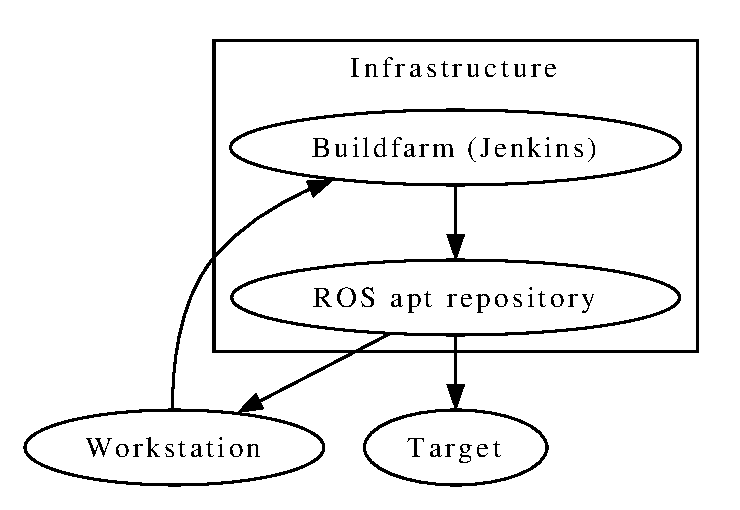
\includegraphics[scale=0.45]{ros.eps}}
    \end{column}
    \begin{column}{.49\textwidth}
        \begin{block}{Highlights}
            \begin{itemize}
                \item everything is package
                \item focus on individual packages (Lego blocks)
                \item deployments delayed in time
            \end{itemize}
        \end{block}
        \begin{block}{\texttt{buildfarm}}
            \begin{itemize}
                \item devel / release jobs
                \item automated testing and rebuilds of dependencies
                \item \texttt{dev} and \texttt{dbg} packages
            \end{itemize}
        \end{block}
    \end{column}
    \end{columns}
\end{frame}

\begin{frame}
    \frametitle{Industrial setup}

    \center{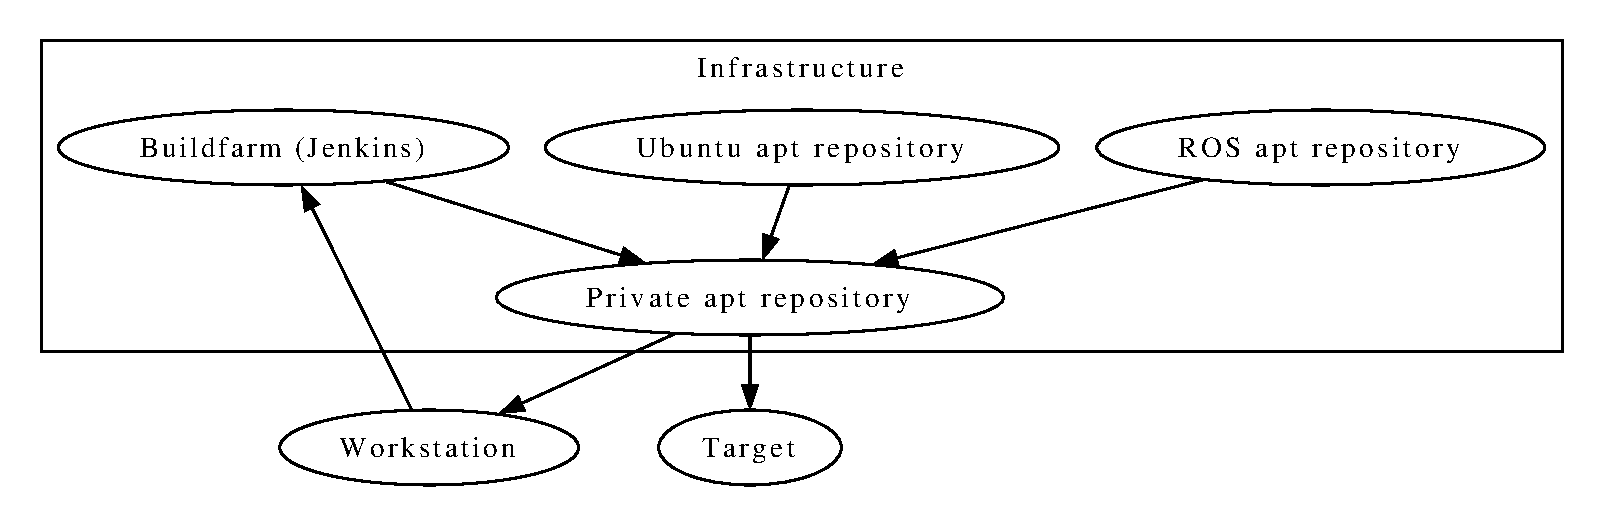
\includegraphics[scale=0.45]{buildfarm.eps}}

    \begin{block}{}
        \begin{itemize}
            \item stable / staging packages
            \item global releases, e.g., to match \texttt{ROS} versions
            \item binary package proxy, e.g., \url{https://aptly.info/}
        \end{itemize}
    \end{block}
\end{frame}

\begin{frame}
    \frametitle{Problems}

    \begin{block}{Industrial requirements}
        \begin{itemize}
            \item fast/parallel deployments needed for tests
            \item system-focused: packages are secondary
        \end{itemize}
    \end{block}

    \begin{block}{Complexity}
        \begin{itemize}
            \item dedicated DevOps
            \item micromanagement: tags, changelogs, release tracks
            \item useless steps, e.g., source package generation
        \end{itemize}
    \end{block}
\end{frame}

\subsection{Workspaces}
\begin{frame}[fragile]
    \frametitle{Workspace -- a project working directory}

    \center{\scriptsize{\url{https://colcon.readthedocs.io/en/released/user/what-is-a-workspace.html}}}

    \begin{block}{Source space}
        \begin{itemize}
            \item repository list and sources
\small{
\begin{verbatim}
repositories:
    intrometry:
        type: git
        url: https://github.com/asherikov/intrometry.git
        version: main
...
\end{verbatim}}
        \end{itemize}
    \end{block}

    \begin{block}{Build space}
        \begin{itemize}
            \item \texttt{cmake} build directories
        \end{itemize}
    \end{block}

    \begin{block}{Install space}
        \begin{itemize}
            \item installation root directory
        \end{itemize}
    \end{block}
\end{frame}

\begin{frame}
    \frametitle{Workspace usage scenarios}

    \begin{block}{Sliding window}
        \begin{itemize}
            \item subset of stack packages
            \item the rest via binary packages
            \item implement feature, release, throw away
            \item \texttt{vcstool} approach
        \end{itemize}
    \end{block}

    \begin{block}{Persistent}
        \begin{itemize}
            \item same set of packages (possibly all)
            \item multiple features in parallel
            \item fork source space, implement feature, merge
            \item more suitable for industrial applications (system focus)
        \end{itemize}
    \end{block}
\end{frame}

\begin{frame}
    \frametitle{Quick deployments}

    \begin{columns}[T]
        \begin{column}{.29\textwidth}
            \center{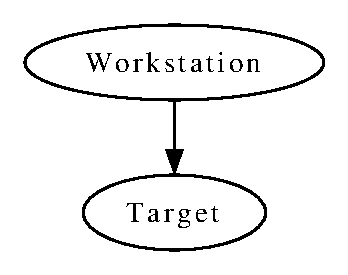
\includegraphics[scale=0.45]{quickie.eps}}
        \end{column}
        \begin{column}{.69\textwidth}
            \begin{block}{Highlights}
                \begin{itemize}
                    \item no common well-defined approach
                    \item copy install workspaces
                        \begin{itemize}
                            \item \texttt{scp}
                            \item \texttt{docker} containers
                        \end{itemize}
                    \item insecurity, fragility
                    \item target architecture may be different
                    \item usually combined with binary packages
                \end{itemize}
            \end{block}

            \begin{block}{\texttt{CCWS} approach (opt-in)}
                \begin{itemize}
                    \item workspace = a single binary package
                        \begin{itemize}
                            \item system-focus
                            \item compact
                            \item parallel installations
                        \end{itemize}
                \end{itemize}
            \end{block}
        \end{column}
    \end{columns}
\end{frame}


\begin{frame}
    \frametitle{Packages are good!}
    \begin{block}{}
        \begin{itemize}
            \item code reuse
            \item installation fine-tuning
            \item nodes/services -- safety via process isolation
            \item rely on dependency management tools (vs. \texttt{cmake})
        \end{itemize}
    \end{block}

    \center{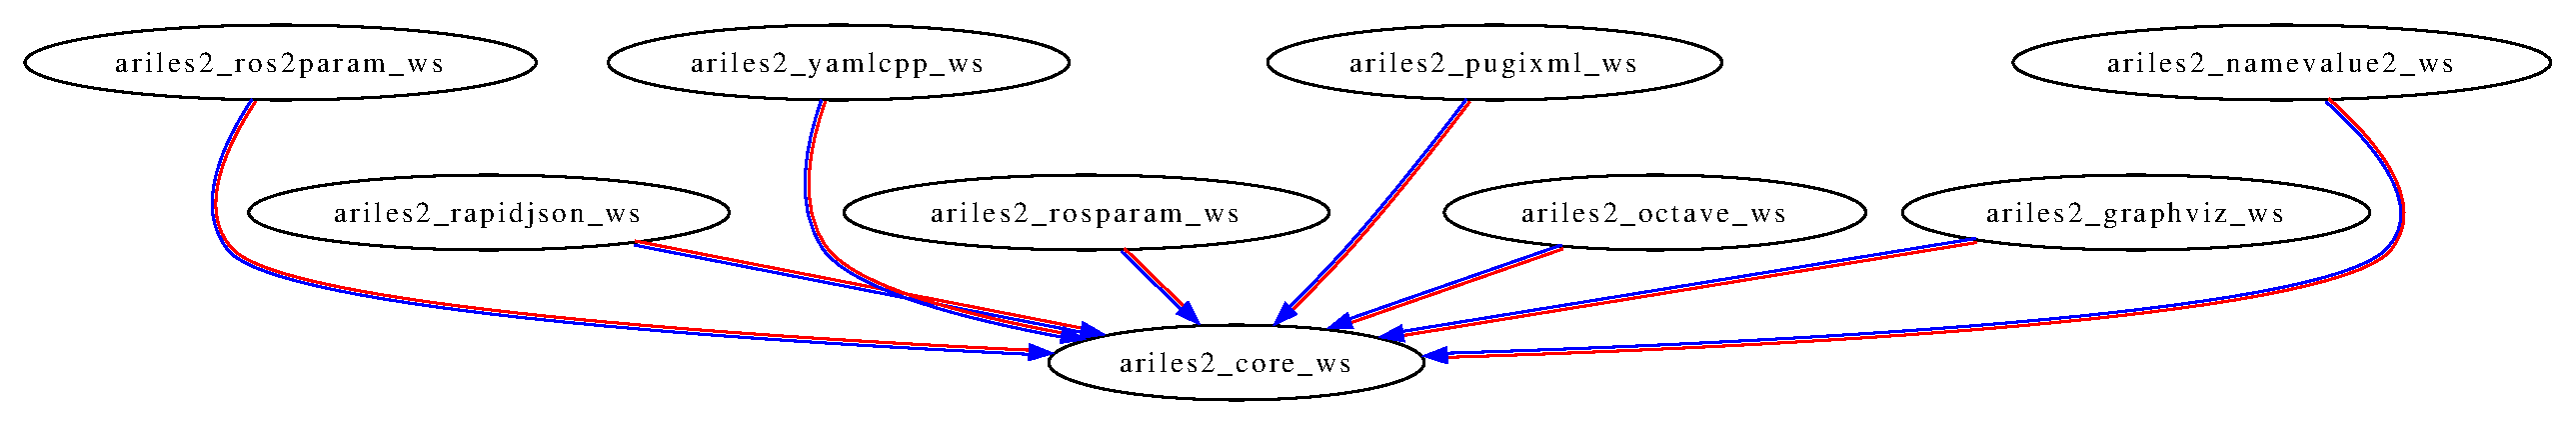
\includegraphics[scale=0.28]{ariles.eps}}
\end{frame}


%%%%%%%%%%%%%%%%%%%%%%%%%%%%%%%%%%%%%%%%%%%%%%%%%%%%%%%%%%%%%%%%%%%%%%%%%%%%%%%
%%%%%%%%%%%%%%%%%%%%%%%%%%%%%%%%%%%%%%%%%%%%%%%%%%%%%%%%%%%%%%%%%%%%%%%%%%%%%%%
%%%%%%%%%%%%%%%%%%%%%%%%%%%%%%%%%%%%%%%%%%%%%%%%%%%%%%%%%%%%%%%%%%%%%%%%%%%%%%%
\section{Implementation}

\begin{frame}
    \frametitle{Under the hood}

    \begin{block}{Implementation}
        \begin{itemize}
            \item[] \texttt{make}
            \item[] \texttt{bash}
            \item[] \texttt{cmake}
        \end{itemize}
    \end{block}

    \begin{block}{3rd party tools}
        \begin{itemize}
            \item[] \texttt{colcon}
            \item[] \texttt{rosdep}
            \item[] \url{https://github.com/asherikov/wshandler} (not \texttt{vcstool})
            \item[] \texttt{cmake}, \texttt{ccache}
            \item[] \texttt{proot}, \texttt{qemu}
            \item[] system utilities: \texttt{mount}, \texttt{losetup}, \texttt{sed}, ...
            \item[] compilers, linters, \texttt{doxygen}
        \end{itemize}
    \end{block}
\end{frame}

\begin{frame}[fragile]
    \frametitle{Directory layout}

    \begin{block}{\texttt{<CCWS root>}}
\small{
\begin{verbatim}
    setup.bash
    Makefile
    ccws
        profiles
        examples
        make
\end{verbatim}}
    \end{block}

    \begin{block}{\texttt{<cache> = [\$XDG\_CACHE\_HOME]}}
\small{
\begin{verbatim}
    ccache
\end{verbatim}}
    \end{block}

    \begin{block}{\texttt{<workspace root> = [<CCWS root>]}}
\small{
\begin{verbatim}
    src
        .ccws
    install/<build profile>
    artifacts/<build profile>
    build/<build profile>
\end{verbatim}}
    \end{block}
\end{frame}

\begin{frame}
    \frametitle{Profiles}

    \begin{block}{Build}
        \begin{description}
            \item[\it{required:}] shell setup script
            \item[\it{optional:}] \texttt{cmake} toolchain
            \item[\it{optional:}] \texttt{Makefile} targets: dependencies, building
        \end{description}
    \end{block}

    \begin{block}{Execution}
        \begin{description}
            \item[\it{required:}] shell setup script
                \begin{itemize}
                    \item generic alternative to \texttt{catkin} hooks
                \end{itemize}
            \item[\it{optional:}] \texttt{Makefile} targets: dependencies
        \end{description}
    \end{block}
\end{frame}

\begin{frame}
    \frametitle{Distributed profiles}

    \begin{columns}[T]
    \begin{column}{.49\textwidth}
        \begin{block}{Build}
            \begin{itemize}
                \item \texttt{reldebug} (\texttt{RelWithDebInfo})
                \item \texttt{scan\_build}: \texttt{clang} + \texttt{scan\_build} + \texttt{clang-tidy}.
                \item \texttt{thread\_sanitizer}
                \item \texttt{addr\_undef\_sanitizers}
                \item \texttt{static\_checks}
                \item \texttt{doxygen}
                \item \texttt{cross\_raspberry\_pi}
                \item \texttt{clangd}
                \item \texttt{deb}
            \end{itemize}
        \end{block}
    \end{column}
    \begin{column}{.49\textwidth}
        \begin{block}{Execution}
            \begin{itemize}
                \item \texttt{common} -- a set of common ROS parameters
                \item \texttt{test}
                \item \texttt{valgrind}
                \item \texttt{core\_pattern}
                \item \texttt{address\_sanitizer}
            \end{itemize}
        \end{block}
    \end{column}
    \end{columns}
\end{frame}

\begin{frame}
    \frametitle{Customization}

    \begin{block}{Global}
        \begin{itemize}
            \item vendor name, paths, default profiles
        \end{itemize}
    \end{block}

    \begin{block}{Profile}
        \begin{itemize}
            \item custom profiles
            \item simple inheritance
        \end{itemize}
    \end{block}

    \begin{block}{Workspace (source space)}
        \begin{itemize}
            \item \texttt{cmake} toolchains
            \item package exceptions and selection
            \item \texttt{Dockerfile}
        \end{itemize}
    \end{block}

    \begin{block}{Package}
        \begin{itemize}
            \item \texttt{CCWS} flags and defines are opt-in
        \end{itemize}
    \end{block}
\end{frame}


%%%%%%%%%%%%%%%%%%%%%%%%%%%%%%%%%%%%%%%%%%%%%%%%%%%%%%%%%%%%%%%%%%%%%%%%%%%%%%%
%%%%%%%%%%%%%%%%%%%%%%%%%%%%%%%%%%%%%%%%%%%%%%%%%%%%%%%%%%%%%%%%%%%%%%%%%%%%%%%
%%%%%%%%%%%%%%%%%%%%%%%%%%%%%%%%%%%%%%%%%%%%%%%%%%%%%%%%%%%%%%%%%%%%%%%%%%%%%%%
\section{Usage}

\begin{frame}[fragile]
    \frametitle{Usage}
\begin{block}{// install \texttt{CCWS} dependencies}
\begin{verbatim}
    make bp_install_build BUILD_PROFILE=reldebug
\end{verbatim}
\end{block}

\begin{block}{// setup repositories}
\begin{verbatim}
    nvim ./src/.repos
    make wsupdate
\end{verbatim}
\end{block}

\begin{block}{// install package dependencies}
\begin{verbatim}
    make dep_install PKG=<MY_PACKAGE>
\end{verbatim}
\end{block}

\begin{block}{// build and test}
\begin{verbatim}
    make <MY_PACKAGE>
    make test_with_deps PKG=<MY_PACKAGE>
\end{verbatim}
\end{block}
\end{frame}


%%%%%%%%%%%%%%%%%%%%%%%%%%%%%%%%%%%%%%%%%%%%%%%%%%%%%%%%%%%%%%%%%%%%%%%%%%%%%%%
%%%%%%%%%%%%%%%%%%%%%%%%%%%%%%%%%%%%%%%%%%%%%%%%%%%%%%%%%%%%%%%%%%%%%%%%%%%%%%%
%%%%%%%%%%%%%%%%%%%%%%%%%%%%%%%%%%%%%%%%%%%%%%%%%%%%%%%%%%%%%%%%%%%%%%%%%%%%%%%
\section{Binary packages}

\begin{frame}[fragile]
    \frametitle{Building and using \texttt{debian} packages}
\begin{block}{// build}
\begin{verbatim}
    make BUILD_PROFILE=deb BASE_BUILD_ROFILE=reldebug
\end{verbatim}
\end{block}

\begin{block}{// install}
\begin{verbatim}
    apt install ./artifacts/deb/ccws__reldebug__staging.deb
\end{verbatim}
\end{block}

\begin{block}{// use}
\begin{verbatim}
    source /opt/ccws/ccws__reldebug__staging/ccws_setup.bash
    ...
\end{verbatim}
\end{block}
\end{frame}


\begin{frame}[fragile]{Binary packages}
    \begin{block}{\texttt{deb} profile}
\footnotesize{
\begin{verbatim}
   make <PKG> BUILD_PROFILE=deb BASE_BUILD_PROFILE=thread_sanitizer
   make <PKG> BUILD_PROFILE=deb BASE_BUILD_PROFILE=cross_raspberry_pi
\end{verbatim}
}
    \end{block}

    \begin{block}{``Superpackages''}
        \begin{itemize}
            \item workspace in a single \texttt{debian} package
            \item all dependencies are resolved and added
            \item simple copy and install
            \item name and path versioning for parallel installation
            \item containerization agnostic
        \end{itemize}
    \end{block}
\end{frame}


\begin{frame}[fragile]
    \frametitle{Package metainformation}
\begin{block}{}
\begin{verbatim}
    dpkg -I artifacts/deb/ccws__reldebug__staging.deb
\end{verbatim}
\end{block}
\small{
\begin{verbatim}
 new Debian package, version 2.0.
 size 3898618 bytes: control archive=728 bytes.
     523 bytes,     7 lines      control
     392 bytes,    13 lines   *  postinst             #!/bin/sh
     173 bytes,     4 lines   *  postrm               #!/bin/sh
     179 bytes,     4 lines   *  preinst              #!/bin/sh
     343 bytes,    13 lines   *  prerm                #!/bin/sh
 Package: ccws--reldebug--staging
 Version: 20241023-2016-humble-3da1ff
 Architecture: amd64
 Maintainer: Alexander Sherikov <alexander@sherikov.net>
 Description: ccws thread_supervisor ariles2_core_ws ...
 Depends: cmake,libboost-all-dev,libeigen3-dev,libgtest-dev ...
 Installed-Size: 8604
\end{verbatim}
}
\end{frame}


\begin{frame}{\texttt{Debian} packages}

    \begin{block}{Pre-install checks}
        \begin{itemize}
            \item system version \texttt{os-release}
            \item conflicts
        \end{itemize}
    \end{block}

    \begin{block}{System configuration}
        \begin{itemize}
            \item \texttt{systemd} services and units
            \item configuration files
            \item udev rules
            \item ssh keys
        \end{itemize}
    \end{block}

    \begin{block}{Simulation packages}
        \begin{itemize}
            \item demos and presentations
        \end{itemize}
    \end{block}
\end{frame}


%%%%%%%%%%%%%%%%%%%%%%%%%%%%%%%%%%%%%%%%%%%%%%%%%%%%%%%%%%%%%%%%%%%%%%%%%%%%%%%
%%%%%%%%%%%%%%%%%%%%%%%%%%%%%%%%%%%%%%%%%%%%%%%%%%%%%%%%%%%%%%%%%%%%%%%%%%%%%%%
%%%%%%%%%%%%%%%%%%%%%%%%%%%%%%%%%%%%%%%%%%%%%%%%%%%%%%%%%%%%%%%%%%%%%%%%%%%%%%%
\section{Cross-compilation}

\begin{frame}{Overview}
    \begin{block}{Approaches}
        \begin{itemize}
            \item emulated compilation
            \item cross-compilation (does not work)
            \item mixed approach: \texttt{proot} + \texttt{qemu}
        \end{itemize}
    \end{block}

    \begin{block}{Challenges}
        \begin{itemize}
            \item cross-compiler is available from packages
            \item reflect development and deployment root filesystems
            \item absolute paths
                \begin{itemize}
                    \item in \texttt{cmake} files
                    \item symbolic links in root filesystems
                \end{itemize}
            \item code generation, embedded scripts, custom compilers
                \begin{itemize}
                    \item \texttt{nvcc}, \texttt{protobuf}, \texttt{ROS} messages
                    \item host vs target
                \end{itemize}
        \end{itemize}
    \end{block}
\end{frame}

\begin{frame}{Obtaining root filesystems}
    \begin{block}{Container-less}
        \begin{itemize}
            \item sources
                \begin{itemize}
                    \item download OS image (Raspberry Pi)
                    \item generate image (NVidia Jetson)
                    \item copy filesystem from the target
                \end{itemize}
            \item modifications and versioning
        \end{itemize}
    \end{block}

    \begin{block}{Docker}
        \begin{itemize}
            \item export container image
            \item modifications are difficult to reflect back
        \end{itemize}
    \end{block}
\end{frame}


\section{Performance}

\begin{frame}{Performance}
    \begin{block}{Rebuilding}
        \begin{itemize}
            \item no prebuilt individual binary packages $\Rightarrow$
                longer build times
        \end{itemize}
    \end{block}

    \begin{block}{Tools}
        \begin{itemize}
            \item \texttt{cmake}
                \begin{itemize}
                    \item not relocatable
                \end{itemize}
            \item \texttt{ccache}
                \begin{itemize}
                    \item compiler wrapper
                    \item object file cache
                    \item up to $\times30$ faster
                    \item can be mounted inside containers
                    \item network-based alternatives
                \end{itemize}
        \end{itemize}
    \end{block}
\end{frame}

\begin{frame}[fragile]{Emulated build}
    \begin{block}{Docker container, 26 packages}
        \vspace{3mm}
        \begin{columns}[T]
            \begin{column}{.3\textwidth}
                clean build
\begin{verbatim}
real  96m32.183s
user  398m2.503s
sys   10m21.164s
\end{verbatim}
            \end{column}
            \begin{column}{.3\textwidth}
                \texttt{ccache} + \texttt{cmake}
\begin{verbatim}
real  9m41.339s
user  9m16.048s
sys   1m8.795s
\end{verbatim}
$\times 10$ faster
            \end{column}
            \begin{column}{.3\textwidth}
                \texttt{ccache}
\begin{verbatim}
real  34m34.321s
user  77m28.042s
sys   3m32.501s
\end{verbatim}
$\times 3$ faster
            \end{column}
        \end{columns}
    \end{block}

    \begin{block}{}
        Not much faster due to \texttt{ROS} messages...
    \end{block}
\end{frame}


\begin{frame}[fragile]{Cross-compilation}
    \begin{block}{includes \texttt{debian} package generation (\texttt{4m55.386s})}
        \vspace{3mm}
        \begin{columns}[T]
            \begin{column}{.3\textwidth}
                clean build
\begin{verbatim}
real  34m55.960s
user  44m21.763s
sys   23m37.602s
\end{verbatim}
$\times 3$ faster
            \end{column}
            \begin{column}{.3\textwidth}
                \texttt{ccache} + \texttt{cmake}
\begin{verbatim}
real  9m6.039s
user  6m6.220s
sys   2m51.399s
\end{verbatim}
$\times 10$ faster
            \end{column}
            \begin{column}{.3\textwidth}
                \texttt{ccache}
\begin{verbatim}
real  15m22.741s
user  13m12.677s
sys   7m32.062s
\end{verbatim}
$\times 6$ faster
            \end{column}
        \end{columns}
    \end{block}
\end{frame}


%%%%%%%%%%%%%%%%%%%%%%%%%%%%%%%%%%%%%%%%%%%%%%%%%%%%%%%%%%%%%%%%%%%%%%%%%%%%%%%
%%%%%%%%%%%%%%%%%%%%%%%%%%%%%%%%%%%%%%%%%%%%%%%%%%%%%%%%%%%%%%%%%%%%%%%%%%%%%%%
%%%%%%%%%%%%%%%%%%%%%%%%%%%%%%%%%%%%%%%%%%%%%%%%%%%%%%%%%%%%%%%%%%%%%%%%%%%%%%%
\section{Conclusion}

\begin{frame}{Final notes}
    \begin{block}{Smaller \texttt{CCWS} features}
        \begin{itemize}
            \item supports both \texttt{ROS1} and \texttt{ROS2}
            \item new package template
            \item memory based selection of job number
            \item interlinked \texttt{doxygen} documentation with dependency graphs
            \item \texttt{debian} package linting
        \end{itemize}
    \end{block}
\end{frame}

\begin{frame}{May be some day}
    \begin{block}{TODO}
        \begin{itemize}
            \item conceal data
                \begin{itemize}
                    \item stripping libraries and executables
                    \item \texttt{dev} and \texttt{dbg} packages
                \end{itemize}
            \item alternative containerization systems
            \item \texttt{nix} or \texttt{guix}
                \begin{itemize}
                    \item gives control over all dependencies
                    \item non-invasive packaging (manifests)
                    \item channels, e.g., \url{https://github.com/asherikov/guix-sherikov}
                \end{itemize}
        \end{itemize}
    \end{block}
\end{frame}

\begin{frame}

    \centerline{Questions?}

\end{frame}


\begin{withoutheadline}
\begin{frame}[fragile,noframenumbering]
    \frametitle{\texttt{wshandler status}}
\footnotesize{%
\begin{verbatim}
>>> wshandler status .../ccws/src/: git sources ---
Flags: H - version hash mismatch, M - uncommited changes
name              version  actual version              HM repository
----              -------  --------------              -- ----------
ariles            pkg_ws_2 tags/ws-2.3.1-0-ge2748ad4      https://git
intrometry        main     tags/0.1.0-0-ga033cd5-dirty  M https://git
thread_supervisor master   tags/1.1.0-0-gbbf8a09          https://git

<<< wshandler status .../ccws/src/: git sources ---
\end{verbatim}
}
\end{frame}
\end{withoutheadline}

\end{document}
